\documentclass{llncs}

\usepackage{times,graphicx,epsfig,boxedminipage,url,xspace,array}

\begin{document}

\thispagestyle{empty}
\title{Formal Verification of Real-Time Data Processing of the LHC Beam Loss Monitoring System: A Case Study}
\author{Naghmeh Ghafari \inst{1} \and Ramana Kumar \inst{2} \and Jeff Joyce \inst{1}
  \and Bernd Dehning \inst{3} \and Christos Zamantzas \inst{3} }
\institute{Critical Systems Labs, Vancouver, BC, Canada
  \and University of Cambridge, Cambridge, UK
  \and CERN, Geneva, Switzerland}

\pagestyle{plain}

\maketitle

\begin{abstract}

We describe a collaborative effort in which the HOL4 theorem prover is being used to formally verify properties of a structure within the Large Hadron Collider (LHC) machine protection system at the European Organization for Nuclear Research (CERN).
The structure, known as \emph{Successive Running Sums} (SRS), provides input to the decision logic for activating the LHC machine protection system in response to the detection of a dangerous level of beam particle loss.
The use of mechanized logical deduction complements an intensive study of the SRS structure using simulation.
We are especially interested in using logical deduction to obtain a generic result that will be applicable to variants of the SRS structure.
This collaborative effort has individuals with diverse backgrounds ranging from theoretical physics to system safety.
One interesting result is the extent to which the use of a formal method has compelled the stakeholders to clarify intricate details of the SRS structure and behaviour.  

\end{abstract}

\section{Introduction}

The Large Hadron Collider (LHC) at the European Organization for Nuclear Research (CERN) is a high-energy particle accelerator.
It collides beams of protons, where each particle has an energy of 14 TeV, and the results of these collisions are used for high-energy physics research.
In order to reach the required magnetic field strengths, the LHC has superconducting magnets cooled with superfluid helium.
Because the energy of the beams is so high (700 MJ), if even a small fraction of the beam particles leak into the equipment they can cause the superconductors to transition to their normal conducting state.
Such a transition is called a quench.
The consequences of a quench range from several hours of down time (to cool the magnets back down to their superconducting state), to months of repairs (in the case of equipment damage).

The main strategy for protecting the LHC from quenches is the Beam Loss Monitoring System (BLMS), which stops the beams safely if the particle loss exceeds thresholds that are likely to result in a quench. 
At each cycle of the beams around the LHC, the BLMS records and processes thousands of data points in order to decide whether to stop the beams.
The processing includes analysis of the loss pattern over time and of the energy of the beam.

The BLMS must respond to dangerous losses quickly, but determining whether losses are dangerous may require analysis of the data recorded over a long period. 
Furthermore, the BLMS must continue recording large amounts of data in real time while processing.
To achieve these goals, the BLMS maintains approximate cumulative sums of particle losses over a variety of sizes of moving windows.
The component responsible for maintaining these sums is called the Successive Running Sums (SRS) structure.
The SRS is implemented in hardware, in order to be fast enough to work in real time, and on FPGAs in particular so that they can be easily reprogrammed with future designs if necessary.
Multiple implementations of the SRS structure are installed regularly around the LHC as part of the BLMS.
<this paragraph probably needs some references>

<SPECIFICATION/REQUIREMENTS OF SRS: it is approximate sums of loss counts, but they need to be relatively close to the exact sums>
<SIMULATION APPROACH TO ANALYSIS OF SRS>
<FORMAL APPROACH>
{\bf myNote: Add 1) the approach currently taken for the analysis of SRS, 2) the approach we took in this paper for the analysis, 3) the reasons behind that  the goals for this case study 4) the main contributions}

 Rushby's emphasis on the role of mechanized logical deduction as an "implacable skeptic that insists on its human user providing justification" thus rings true.
 %Rushby's description of mechanized logical deduction as an "implacable skeptic that insists on its human user providing justification" rings true for this effort.

The your process of trying to
capture the specification via experiment and refinement by a team with
different backgrounds and expertise is very interesting. the eventual goal is to use HOL4 theorem prover to show
the correctness of the SRS technique in BLM



%The loss of a very small fraction of the circulating beam may induce a quench of the super conducting magnets or even physical damage to machine components. The detection of the lost beam protons allows protection of the equipment against quenches and damage by generating a beam dump trigger when the losses exceed thresholds. At each turn of the beam, there will be several thousands of data to record and process in order to decide if the beams should be permitted to continue circulating or their safe extraction is necessary to be triggered. 

%In general, the BLM system converts the signal given by the recording of shower particles into electrical signals and decides if threshold limits are being exceeded. The beam-permit signal is de-asserted if one detector exceeds the limit and consecutively is transferred to the beam dump system  by the Beam Interlock system.



\section{BLM System Overview}


\begin{figure}[t]
  \centering  \scalebox{0.7}{ 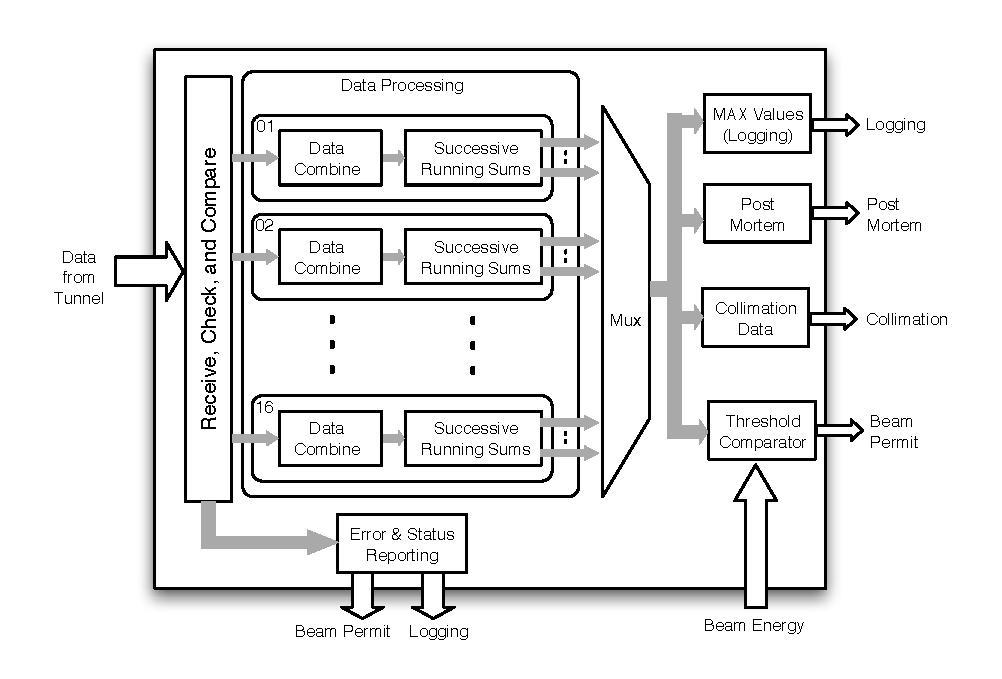
\includegraphics{BLETC.eps}}
   \caption{Block diagram of the processes assigned to BLETC card.}
  \label{fig:BLETC}
\end{figure}

The loss measurement principle \cite{Dehning-IPAC,Chris-FPGA} is based on the energy deposition detection of secondary shower particles using a specially-designed detector called \emph{ionization chamber}. There are around 4000 ionization chambers located under the magnets all around the tunnel. These detectors convert the signal given by the recording of shower particles into electrical signals and send them to tunnel cards. Tunnel cards, which are located in the tunnel and implemented by radiation-tolerant electronics, acquire and digitize the data from the detectors and transmit those to the surface using optical links. There, the data processing cards, named BLETCs, receive those data and decide whether or not the beam should be permitted to be injected or continue circulating. Each tunnel card receives data from eight detectors and each surface card receives data from two tunnel cards. The surface card provides data to the Logging, the Post Mortem and the Collimation systems that will be used to drive on-line displays in the control room to allow offline analysis of the losses and to setup automatically the collimators. Due to demanding performance requirements, the BLM system is making use of modern field programmable gate arrays (FPGAs), which include the resources needed to design complex processing and can be reprogrammed making them ideal for future upgrades or system specification changes. Figure~\ref{fig:BLETC} shows a block diagram of the processes assigned in BLETC FPGA. In the following, we give a brief overview of each of the four main processing blocks in BLETC card. 



\emph{(a) Receive, Check, and Compare (RCC)}: RCC is responsible for facilitating the reception process at the entry stage of the surface FPGA. It ensures the correct reception and detection of erroneous transmissions by redundancy in transmissions and using Cyclic Redundancy Check (CRC) and the 8B/10B algorithms. 

\emph{(b) Data Processing}: Quench of magnets that result from proton loss depends on the loss duration and the beam energy. Given the tolerance acceptable for quench prevention, the quench threshold versus loss time is approximated with a minimum number of sliding integration windows (called \emph{Running Sums}) fulfilling the tolerance. In order to achieve the \emph{dynamic range} (i.e. the domain of variation of the beam losses) requested by the specification, the detectors use both Current-to-Frequency Converters (CFCs) and ADC circuitries. The data processing block merges these two types of data coming from the same detector into one value and send it to Successive Running Sums (SRS) block. The verification of SRS block is the focus of this paper and its implementation is discussed in more detail in the next section. 

\emph{(c) Threshold Comparator}: Every new calculated running sum need to be compared with the corresponding threshold that was chosen by the beam energy reading given that moment. The comparator will initiate a beam dump request if any of the running sums is higher than its corresponding threshold. The beam dump requests are forwarded to the Beam Interlock System which will initiate the beam dump. There are 12 running sums calculated for each 16 detector channels allocated to a BLETC card. The beam energy information is scaled into 32 levels (0.45 to 7 TeV) and each processing module will hold data only for those 16 detectors connected. That would give a total of 6,144 threshold values needed to be held on each card. 

\emph{(d) Logging, Post Mortem and Collimation}:  To be able to trace back the loss signal development, BLM should store the loss measurement data. This data will be sent over the VME-bus for online viewing and storage by the Logging and Post-Mortem systems. For the purpose of supervision, the BLM system will drive an online event display to show error and status information recorded by tunnel electronics and the RCC process as well as the maximum loss rates seen by the running sums. BLETC card also provides data to Collimation system for the correct alignment and setup of the collimators. 




\section{Successive Running Sums (SRS)}

\begin{figure}[t]
  \centering 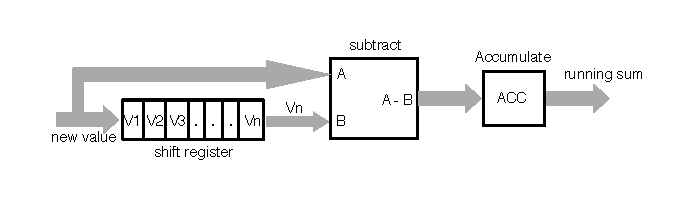
\includegraphics{rs.eps}
   \caption{Block diagram showing how to produce and maintain a continuous running sum of arriving values.}
  \label{fig:RS-basic}
\end{figure}


Beam losses can happen either in a single turn of the beam in the tunnel, with a sudden beam loss, or in progressive losses during numerous turns. One-turn failures are called \emph{ultra-fast} losses. Multi-turn losses can be divided between \emph{very fast} losses those which happen in less than 10 ms, \emph{fast} losses which happen in more than 10 ms and \emph{steady} losses, where the beam is lost over one second or more~\cite{Schmidt-ICFA}.


The processing of the data collected by the detectors involves a proper analysis of the loss patterns in time and a proper account of the energy of the beam. The procedure for the data processing is based on the idea that a constantly updated moving window can be kept by adding to a register the incoming newest value and subtracting its oldest value (see Figure~\ref{fig:RS-basic}). The number of values that are kept under the window defines the integration time it represents.  The ideal strategy is to have an infinite number of constantly updated moving windows with various lengths to cover the whole time region from 40 micro-seconds (the data arrival rate to BLETC card)  to 100 seconds for detecting ultra-fast losses to steady losses, respectively. Such an implementation is not feasible due to the limited amount of resources. Therefore, given the tolerance acceptable for quench prevention, the quench threshold versus loss time curve is approximated by a minimum number of steps that fulfill this tolerance.

\begin{figure}[t]
  \centering 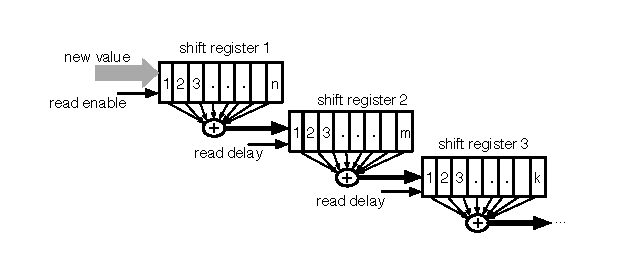
\includegraphics{SRS-basic.eps}
   \caption{Block diagram showing a configuration for efficient summation of many values.}
  \label{fig:SRS-basic}
\end{figure}



In order to construct long moving windows, it is required to keep long histories of received data. The technique employed to reach long integration periods with relatively small in length shift registers uses consecutive storage of sums of the received values. Instead of storing all values needed for the sum, this technique stores successively parts of the total sum using only a fraction of the otherwise needed memory space. This technique works by feeding the sum of one shift register's contents, every time its contents become completely updated, to the input of another shift register (see Figure~\ref{fig:SRS-basic}). By cascading more of these elements, very long moving windows could be constructed with significantly small memory space. The above scheme is the basis for \emph{Successive Running Sums} (SRS) implementation in BLETC. 

SRS implementation minimizes the resource usage by using the already calculated running sums in order to calculate bigger in length running sums without the need of extra summation points. In addition, it makes use of multipoint shift registers that are configured to give intermediate outputs, referred to as \emph{taps}. The taps provide data outputs at certain points in the shift register chain thus contribute towards the efficient use of resources. 


As in the SRS implementation the sum of one shift register's content is fed to the input of another shift register, the optimal achievable latency in the response of each stage is equal to the refreshing time of the preceding shift registers, i.e. the time needed to completely update its contents.  The \emph{read delay} signal (see Figure~\ref{fig:SRS-basic}) of each shift register holds a delay equal to this latency to guarantee the correct operation. Thus, the delay is every time equal to the preceding shift register's delay multiplied by the elements planned to be used in the sum. 

\begin{figure}[t]
  \centering \scalebox{0.65}{ 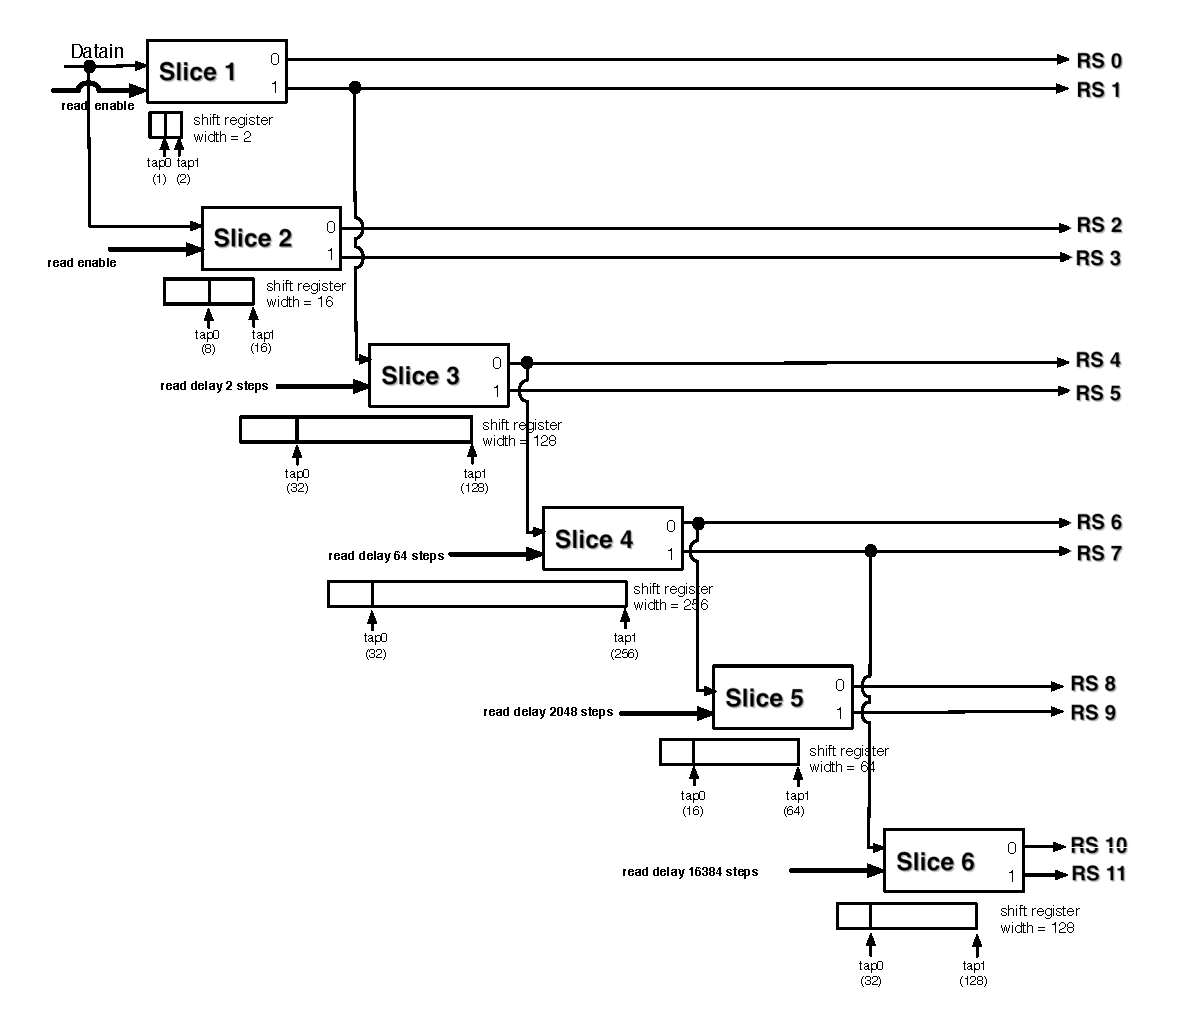
\includegraphics{srs-modified.eps}}
   \caption{The block diagram showing the Successive Running Sums implementation in BLETC card.}
  \label{fig:srs}
\end{figure}


Figure~\ref{fig:srs} shows the implementation of SRS in BLETC card. It consists of 6 \emph{slices}, where each slice computes two running sums (noted by RS) with the use of a multipoint shift register, two subtractors and two accumulators (see Figure~\ref{fig:slice}). 

As shown in Table~\ref{}, by cascading 6 slices, it is enough to reach the 100 seconds upper integration limit requested by the specifications. 

\begin{figure}[t]
  \centering \scalebox{0.8}{ 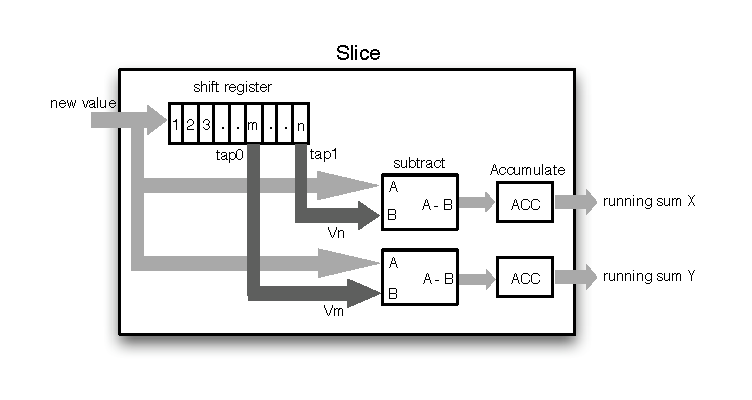
\includegraphics{multi-rs.eps}}
   \caption{The block diagram showing the implementation of each slice.}
  \label{fig:slice}
\end{figure}


\begin{figure}[t]
\centering
\begin{tabular}{|c|c|c|c|c|c|}
\hline
\multicolumn{2}{|c}{Range} &\multicolumn{2}{|c|}{Refreshing} & & \\\cline{1-4}
40 us steps & ms & 40 us steps  & ms & slice No & running sum \\\hline\hline
1 & 0.04 & 1 & 0.04 & & RS0 \\\hline
2 & 0.08 & 1 & 0.04 & & RS1 \\\hline
8 & 0.32 & 1 & 0.04 & slice 1 & RS2 \\\hline
16 & 0.64 & 1 & 0.04 & & RS3 \\\hline
64 & 2.56 & 2 & 0.08 & slice 2 & RS4 \\\hline
256 & 10.24 & 2 & 0.08 & & RS5 \\\hline
2048 & 81.92 & 64 & 2.56 &slice  3 & RS6 \\\hline
16384 & 655.36 & 64 & 2.56 &slice 3 & RS7 \\\hline
32768 &1310.72 & 2048 & 81.92 & slice 4 & RS8 \\\hline
131072 & 5242.88 & 2048 & 81.92 & slice 4 & RS9 \\\hline
524288 & 2097.52 & 16384 & 655.36 & slice 5 &RS10 \\\hline
2097152 & 83886.08 & 16384 & 655.36 & slice 5 & RS11 \\\hline

\end{tabular}
\vspace{0.04in}
\label{fig:example-bakery}
\caption{}
\end{figure}




%A similar configuration for the production of the running sums is used in the BLMTC where in order to increase the efficiency in resources, a set of parameterized multipoint shift registers are used. In this configuration, called \emph{Successive Running Sums}, each incoming new value is delayed with a fixed number of cycles by passing it through a shift register and adding the difference of the new and the outputted from the shift register to an accumulator (see Figure ). 


\section{Verification of SRS Implementation using HOL}

Calculation of the running sums is a critical component of BLM. In case of no dangerous loss, BLM should not inhabit the beam. If it fails, it generates a false alarm and three hours will be lost to recover the previous situation. Such false alarms compromise the availability of the system. Moreover, in case of a dangerous loss, BLM it has to inhibit the beam permit. If it fails there will be at least 30 days of downtime. 
Any error in this computation would either compromise the availability of the system (unnecessary request for beam dump) or safety of the system (nor requesting a necessary beam dump). The current practice to check the correctness of the SRS is by simulation and testing in which (explanation of how such a test gets performed). 

In this paper we present a formal verification approach for the analysis of SRS implementation in BLM.  


The formal verification effort described in this paper is based on
 the use of mechanised logical deduction, or theorem proving, to
 demonstrate that desired properties of a system are logically implied
 by a formal model of the system.  Our approach to theorem-proving
 uses the HOL4 open source software tool, which was developed
 initially at the University of Cambridge, but now by an international
 team~\cite{HOL4}.  HOL4 partially automates the task of proving theorems of
 higher-order logic [ref], a formal logic with a similar expressive
 power to set theory that is widely used for formalising hardware and
 software models and statements about them.  Typically, a very large
 portion of the logical deduction is performed automatically by the
 HOL4 system leaving the user to provide the high level proof
 strategy.  The implementation of the HOL4 system is based on Milner's
 LCF approach [ref] and consists of a small �kernel� that provides a
 very high level of confidence in the logical soundness of the
 verification results obtained using the system. The work described
 here could have been done using other systems such as HOL Light
 [ref], Isabelle/HOL [ref], ProofPower [ref], PVS [ref] or Coq
 [ref]. The first three of these support essentially the same version
 of higher-order logic as HOL4, whilst PVS and Coq support more
 powerful logics. <What about ACL2?>

 While offering less �push button� automation than many other kinds of
 formal verification such as model-checking, machine-assisted theorem
 proving is the most appropriate approach to verifying the BLM SRS,
 since it is unlikely that the correctness theorems, which need lemmas
 proved by manually guided mathematical induction, could be generated
 automatically. 

The main objective of formalizing the functionality of SRS was to keep the topology parameterized. It is very probable that in the future the configuration of the slices and shift registers changes to accommodate higher precision. If the model is parameterized then, the same model can be used in the future uses of the system. For this, we formalized the definitions of the model by six parameters: 



\section{Conclusions and Lessons Learned}



\bibliographystyle{plain} 
\bibliography{refs}


\end{document}

